% siminos/xiong/thesis/proposal/tex/ppt.tex
% $Author: predrag $ $Date: 2015-09-11 18:32:40 -0400 (Fri, 11 Sep 2015) $

%% logical setup, no need to edit %%%%%%%%%%
\newif\ifpaper \newif\ifPDF               %%
\newif\ifOUP \newif\ifboyscout            %%
\newif\ifdasbuch \newif\ifarticle         %%
\newif\ifsolutions

\newif\ifbackground % whether use background image
\backgroundfalse
\newif\iflogo % whether use logo
\logotrue
\newif\ifnotes % whether show notes.
\notesfalse
\newif\ifhandout % handout mode
\handoutfalse
%%%%%%%%%%%%%%%%%%%%%%%%%%%%%%%%%%%%%%%%%%%%%%%%%%%%%%%%%%%%%%%%%%%%%%

\ifhandout
\documentclass[mathserif, handout]{beamer}
\else
\documentclass[mathserif]{beamer}
\fi

\usepackage{graphicx}
\usepackage{algpseudocode}
\usepackage{algorithm}
\usepackage{tikz}
\usetikzlibrary{calc}
\usetikzlibrary{decorations.pathreplacing}
\usepackage{tipa}
\usepackage[font=small,labelfont=bf]{caption}
\usepackage{subcaption}
\usepackage{amsthm}

%%%%%%%%%%%%%%%%%%%%%%%%%%%%%%%%%%%%%%%%%%%%%%%%%%%%%%%%%%%%%%%%%%%%%%
% deal with the conflicts between def.tex and beamer
\newcounter{chapter}
\let\block\undefined
\let\Loop\undefined
\let\definition\undefined
\let\theorem\undefined
\let\lemma\undefined
\input ../../../../inputs/def            %% do not edit; update from
\input ../../../../inputs/defsLyapunov


\graphicspath{{../../../../figs/cqcglFigs/}{../../../../schur/figs/}{../../../figures/}{../../../../schur/ppt/figs/}}

% ------                       setup of beamer               ----------------
\usetheme{Madrid}

\ifnotes
\setbeameroption{show notes}
\else
\setbeameroption{hide notes}
\fi

\setbeamertemplate{bibliography item}[text]
% add background image
\ifbackground
\usebackgroundtemplate
{
  
\includegraphics[width=\paperwidth,height=\paperheight]{./figs/background.jpg}%
}
\fi

% -------------------      title page       --------------------------
\title[Spatio-temporal Chaos] % (optional, only for long titles)
{Recurrent Spatio-temporal Structures}
\subtitle{in Presence of Continuous Symmetries}
\logo{
  \iflogo
  
\includegraphics[width=2cm,height=1cm,keepaspectratio]{gtlogo}
  
\includegraphics[width=1cm,height=0.8cm,keepaspectratio]{cnslogo}
  \fi
}
\author[X. Ding] % (optional, for multiple authors)
{Xiong Ding %\inst{1}
}
\institute[Gatech] % (optional)
{
  % \inst{1}%
  Center for Nonlinear Science \\
  School of Physics \\
  Georgia Institute of Technology
}

\date[Thesis Proposal] % (optional)
{ adviser: Prof. Predrag Cvitanovi\'c \\ \vspace{1em}
  Thesis Proposal, Sep 2015
} %\\ Topics in Geometric and Nonlinear Dynamical Systems}

\subject{Computer Science}

% ----------------    setup of outline    -------------------------
\AtBeginSection[]
{
  \begin{frame}
    \frametitle{Table of Contents}
    \tableofcontents[currentsection]
  \end{frame}
}

% ---------------   main content of slides  -----------------------
\begin{document}
\frame{\titlepage} % add title page.

% ----------------  section: definition of problem --------------

\section{Introduction}

\begin{frame}
  \frametitle{Cycle expansions}
  {\color{cyan} Spatial-temporal averages} can be evaluated
  as a sum over of periodic
  orbits~{\color{blue}[chaosbook.org]} %\color{blue}\cite{DasBuch}}
  \emph{spectral determinant}\rf{CBconverg, pexp}
  \beq
  \det(\eigenvL - \Aop)  \defeq \exp \left(
    - {
      \sum_{p} \sum_{r=1}^\infty {1 \over r}
      {   e^{r (\beta \Obser_p -\eigenvL\period{p}) }
        \over  \oneMinJ{r}}
    }
  \right)
  \label{Z(s)}
  \eeq
  \begin{equation}
    \label{eq:expect}
    \left. \frac{\partial \eigenvL}{\partial \beta_j}
    \right|_{\beta=0} = \expct{\obser_j}
  \end{equation}

  \begin{figure}[h]
    \centering
    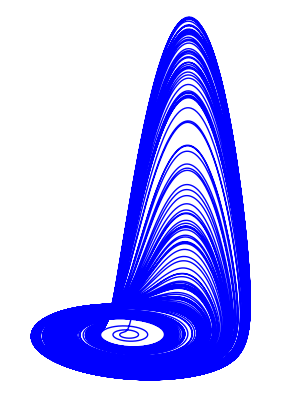
\includegraphics[width=0.11\textwidth]{ergodic} %\hfill
    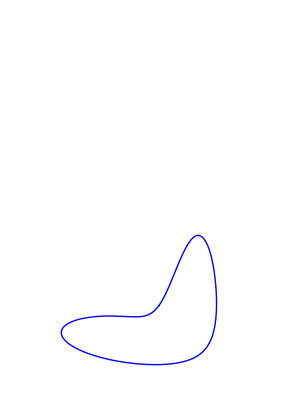
\includegraphics[width=0.11\textwidth]{po1} %\hfill
    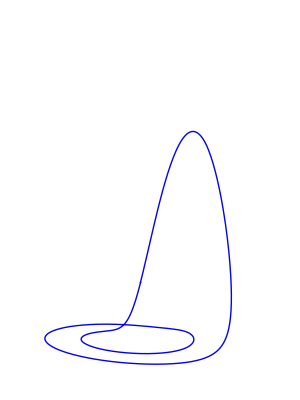
\includegraphics[width=0.11\textwidth]{po2} %\hfill
    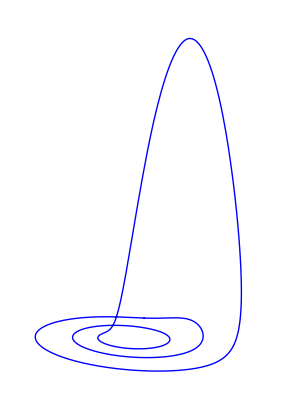
\includegraphics[width=0.11\textwidth]{po3} %\hfill
  \end{figure}

\end{frame}

\begin{frame}
  \frametitle{Global Attractor \& Inertial Manifold\rf{infdymnon}}
  Dissipative dynamical system as a semigroup $\{S(t)\}_{t\ge 0}$ defined in Hilbert space $H$:
  \[
    S(t): u_0 \in H \mapsto u(t) \in H
  \]
  \textbf{Global attractor} : a subset $X \subset H$:
  \begin{equation}
    \label{eq:attractor}
    \begin{align*}
      & S(t) X = X \,,\quad \forall\, t \in \mathbb{R} \\
      & d\left(u(t), X \right) \to 0 \quad t \to \infty
    \end{align*}
  \end{equation}

  \textbf{Inertial Manifold} : a finite dimensional smooth manifold $\mathcal{M} \subset H$
  \begin{equation}
    \label{eq:IM}
    \begin{align*}
      & S(t) \mathcal{M} \subset \mathcal{M} \,,\quad t > 0 \\
      & d\left(u(t), \mathcal{M} \right) \,\le\,  C_1 e^{-C_2 t}
    \end{align*}
  \end{equation}

\end{frame}

\begin{frame}
  \frametitle{  \cLv\ algorithm\rf{GiChLiPo12}}

  \input ../../../../schur/ppt/figCLV

\end{frame}

\begin{frame}
  \frametitle{  \psd \rf{Bojanczyk92theperiodic}}
  \begin{figure}[h]
    \centering
    
\includegraphics[width=0.5\textwidth]{per_schur_algorithm.pdf}
  \end{figure}

\end{frame}

\begin{frame}
  \frametitle{ \scriptsize{1-dimensional \cqcGLe\rf{cross93}} }

  \begin{equation}
    \label{eq:cqcgl1d}
    A_t = \mu A + DA_{xx} + \beta |A|^2A + \gamma |A|^4A \,,\quad x\in[0,L]
    \,.
  \end{equation}

  Intermittent explosion in soliton solution:
  \begin{figure}[h]
    \centering
    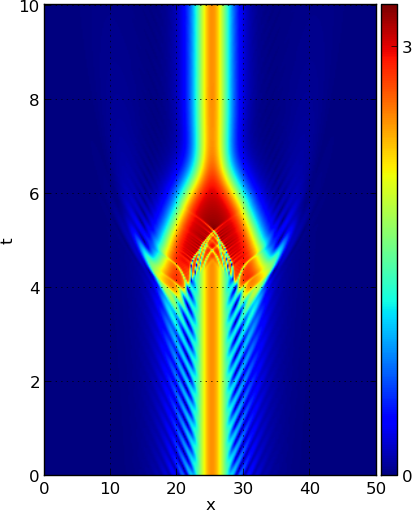
\includegraphics[width=0.33\textwidth]{symmetricExplosion}%\hfill
    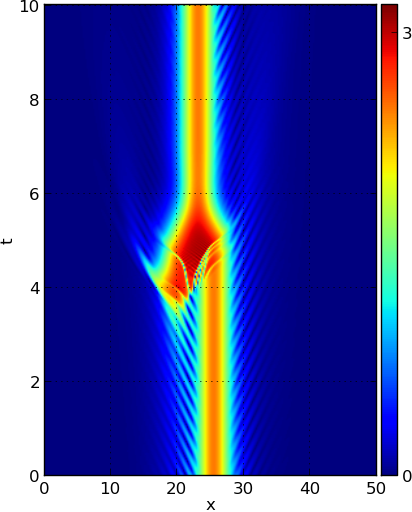
\includegraphics[width=0.33\textwidth]{asymmetricExplosion1}%\hfill
    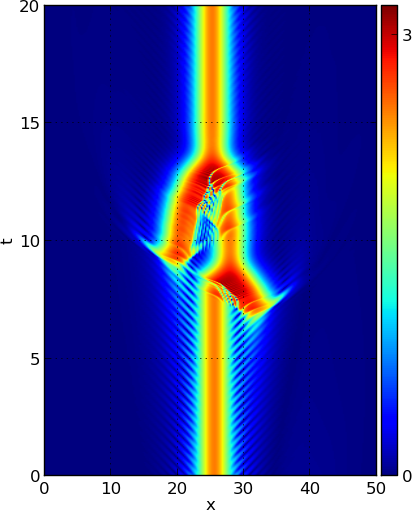
\includegraphics[width=0.33\textwidth]{asymmetricExplosion2}
    \label{fig:explosionTypes}
  \end{figure}

\end{frame}
% -------      section: periodic eigendecomposition ----------
\section{Preliminary Results}

\begin{frame}[allowframebreaks]
  \frametitle{Computing \Fv s\rf{DingCvit14}}

  1-dimensional \KSe\ :
  a flame on a ring, with the flame velocity satisfying
  \[
    u_t+\frac{1}{2}(u^2)_x+u_{xx}+u_{xxxx}=0\,,\quad x\in [0,L]
  \]
  In our simulations $L=22$.
  \begin{figure}[h]
    \centering
    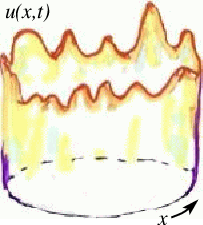
\includegraphics[width=0.3\textwidth]{flameFlut}
  \end{figure}


  \begin{figure}[h]
    \centering
    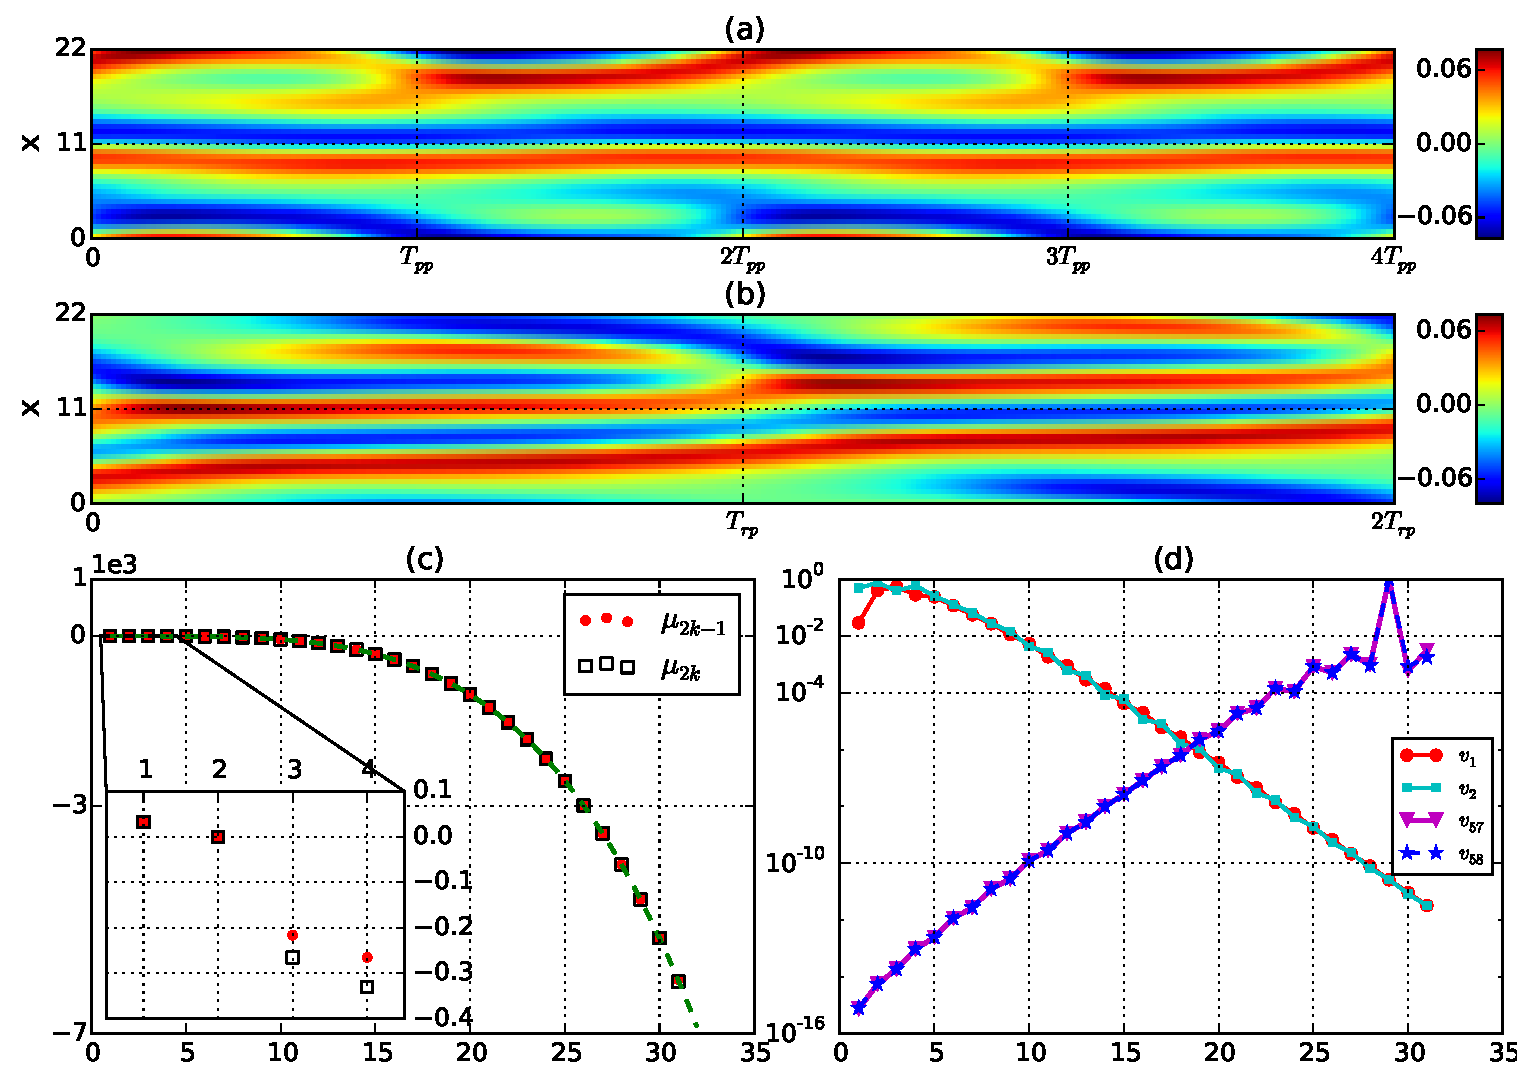
\includegraphics[width=0.9\linewidth]{pprpfigure}
    \label{fig:ppo1state}
  \end{figure}

  \begin{table}[h]
    \footnotesize
    \centering
    \caption{
      The first 10 and last four Floquet exponents and
      Floquet multiplier phases,
      $ \ExpaEig_i= \exp(\period{}\,\eigRe[i] \pm i\theta_{i})$, for
      orbits $\cycle{pp}_{10.25}$ and $\cycle{rp}_{16.31}$, respectively.
    }
    \label{tab:floquet_ppo1}
    \begin{tabular}{l l c | l l c}
      \multicolumn{3}{c |}{$\cycle{pp}_{10.25}$} & \multicolumn{3}{c}{$\cycle{rp}_{16.31}$}\\
      $i$ & ~~~~~$\eigRe[i]$  & $\theta_{i}$  & $i$ & ~~~~~$\eigRe[i]$ & $\theta_{i}$  \\
      \hline
      1,2 & ~0.033209  &    $\pm$2.0079  &  1 &     ~0.32791  &              \\
      3 & -4.1096e-13  &                 &  2 &   ~2.8679e-12  &              \\
      4 & -3.3524e-14  &    -1           &  3 &   ~2.3559e-13  &              \\
      5 &  -0.21637    &                 &  4 &     -0.13214  &        -1    \\
      6,7 &  -0.26524  &   $\pm$2.6205   &  5,6 &   -0.28597  & $\pm$2.7724  \\
      8 &  -0.33073    &    -1           &  7 &     -0.32821  &       -1     \\
      9 &  -1.9605    &                  &  8 &      -0.36241  &             \\
      10 & -1.9676    &    -1            &  9,10 &   -1.9617  &  $\pm$2.2411 \\
      $\cdots$ &  $\cdots$    & $\cdots$ & $\cdots$ & $\cdots$ & $\cdots$   \\
      59 &  -5313.6   &    -1           &  59 &   -5314.4 &                 \\
      60 &  -5317.6   &                 &  60 &   -5317.7 &                 \\
      61 &  -6051.8   &    -1           &  61 &   -6059.2 &                 \\
      62 &  -6080.4   &                 &  62 &   -6072.9 &                 \\
      \hline
    \end{tabular}
  \end{table}

  \begin{figure}[h]
    \centering
    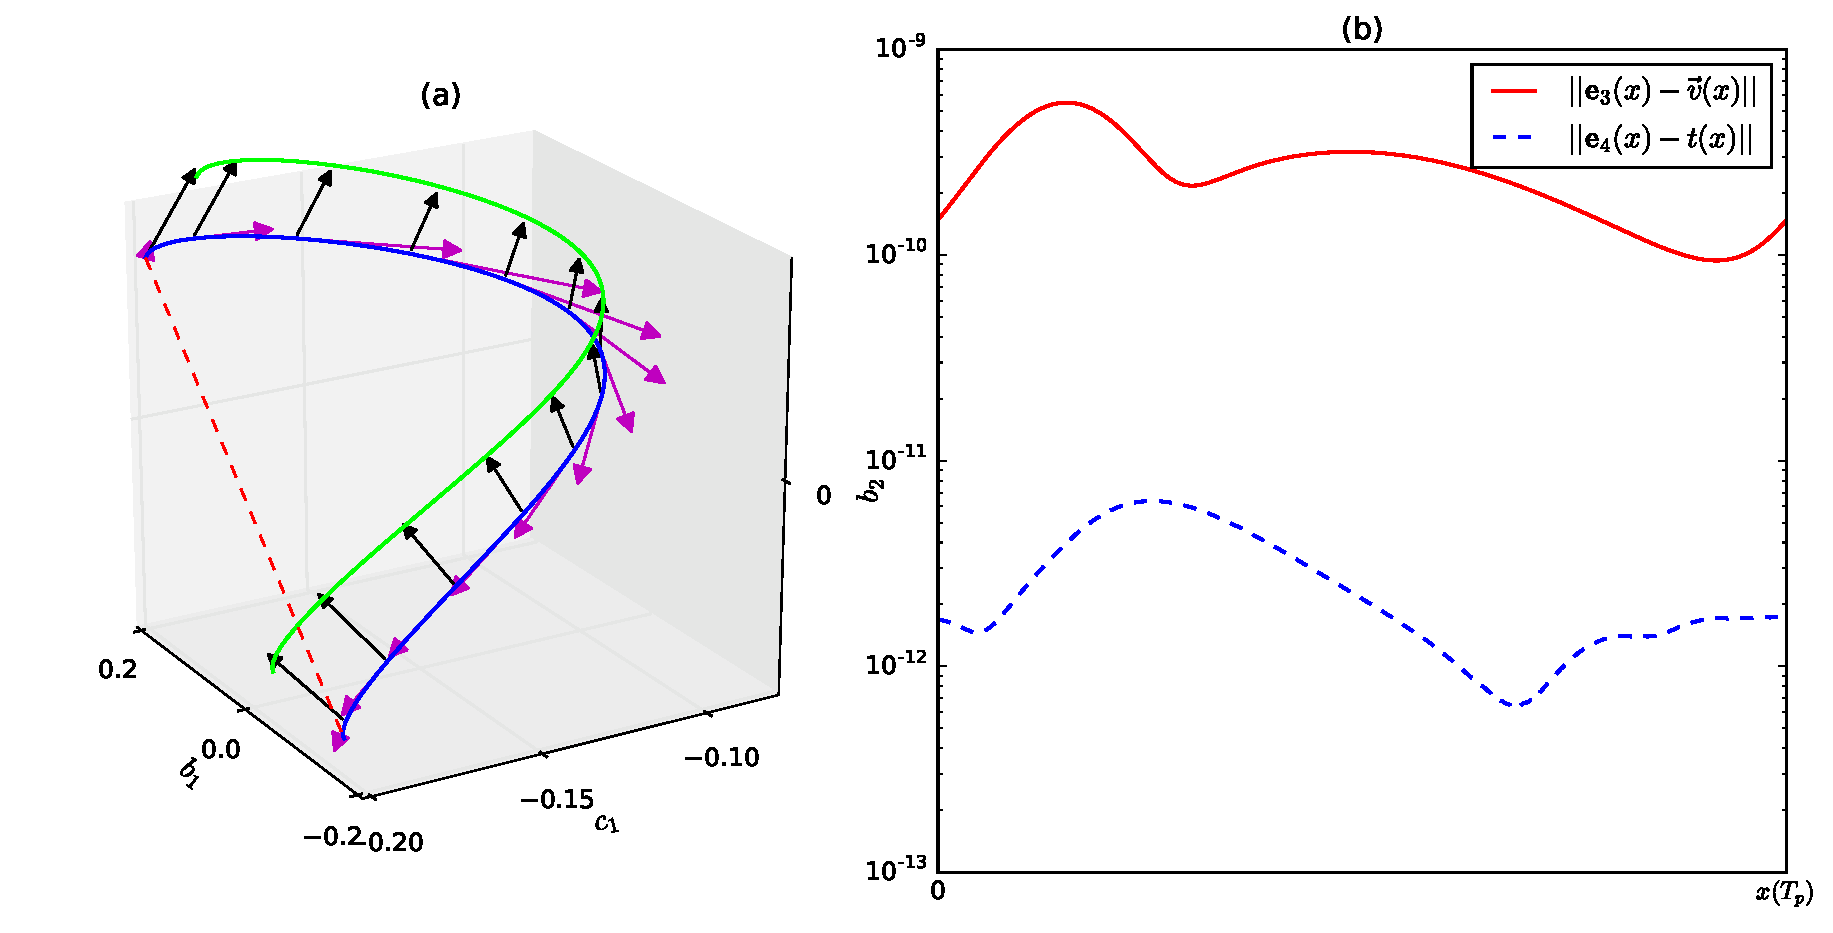
\includegraphics[width=1.0\linewidth]{ppo1vectfield}
    \label{fig:ppo1vectorfield}
  \end{figure}

  \begin{figure}[h]
    \centering
    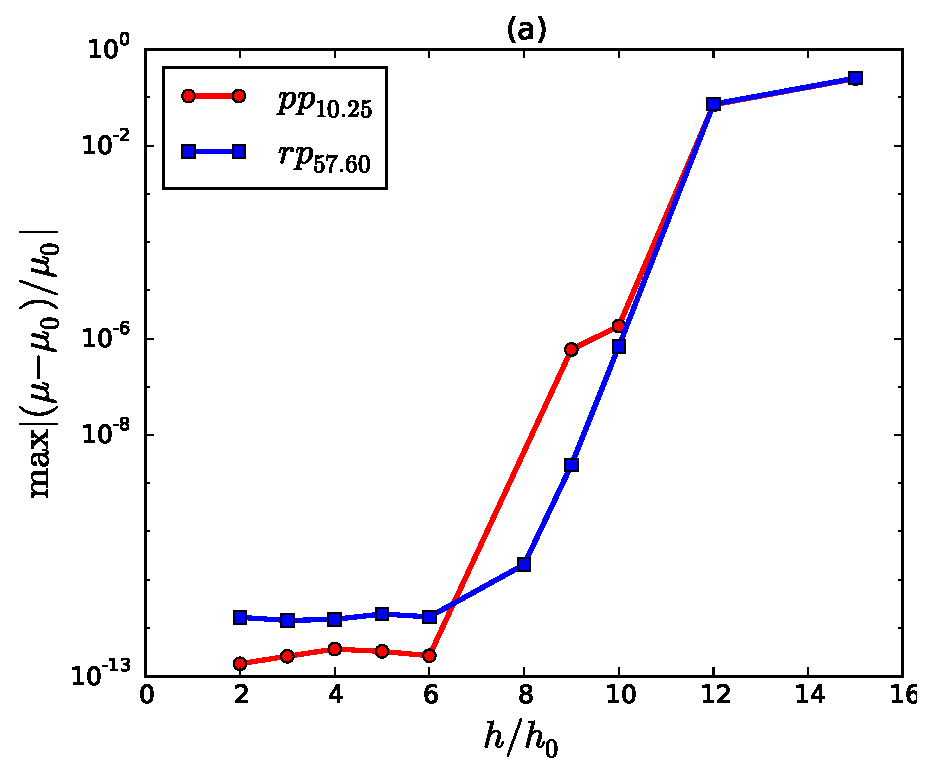
\includegraphics[width=0.47\linewidth]{ppo1FEerror} \hfill
    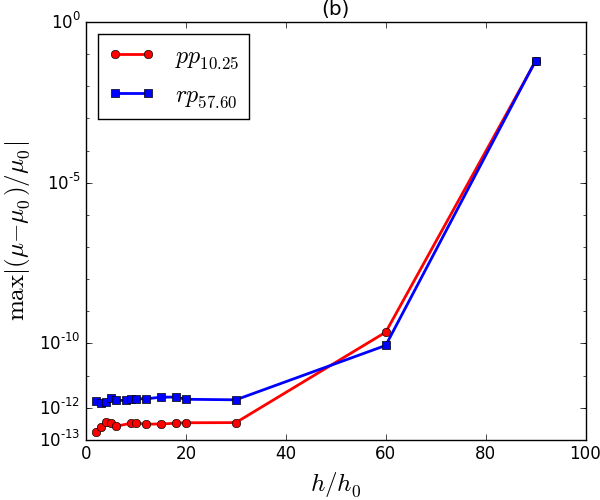
\includegraphics[width=0.47\linewidth]{rpo22FEerror}
    \label{fig:FEerror}
  \end{figure}

\end{frame}

\begin{frame}[allowframebreaks]
  \frametitle{Local expansion of Inertial Manifold by Floquet Vectors}

  \begin{figure}[h]
    \centering
    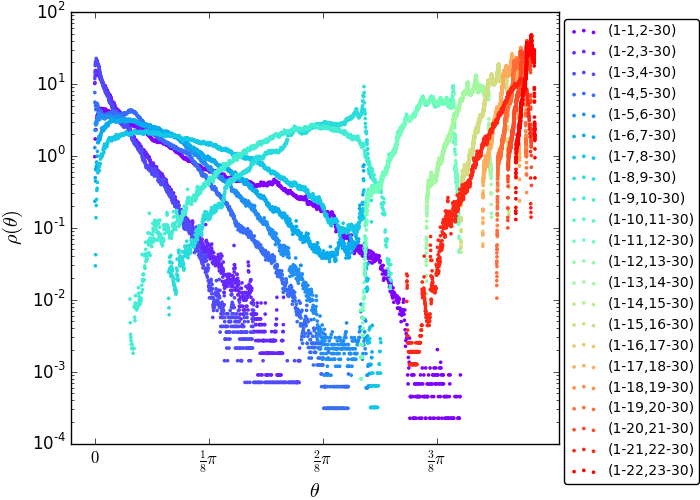
\includegraphics[width=0.48\textwidth]{angle120ppoSpace1} \hfill
    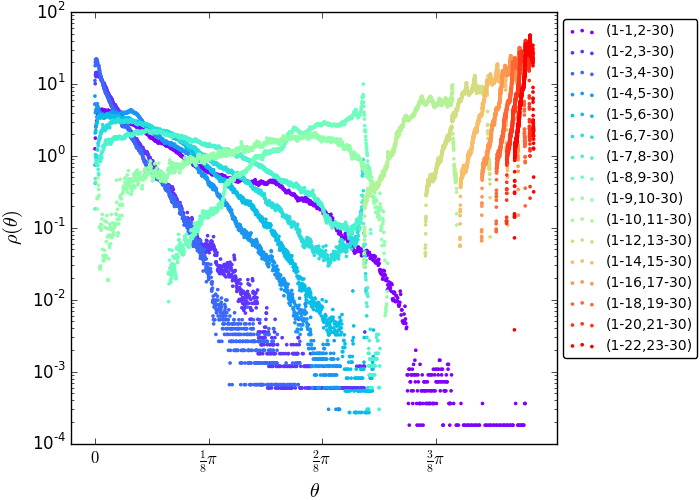
\includegraphics[width=0.48\textwidth]{angle120rpoSpace1}
    \caption{Angle distribution $\rho(\theta)$ versus $\theta$
      for \cycle{ppo} (left) and \cycle{rpo} which has $ T < 120$.
    }
    \label{fig:angDist}
  \end{figure}

  \begin{figure}[h]
    \centering
    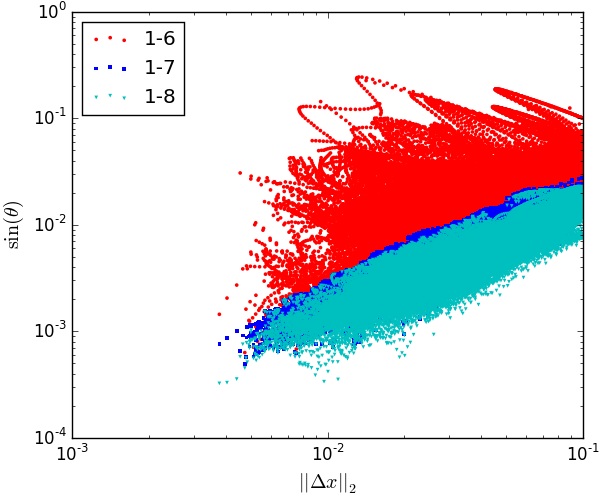
\includegraphics[width=0.48\textwidth]{ppo3truncated} \hfill
    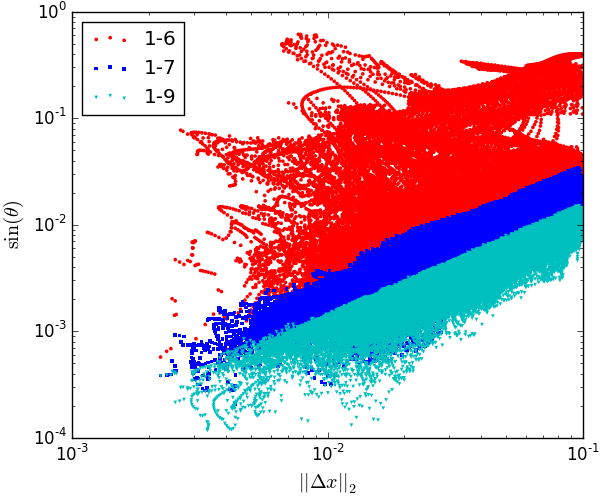
\includegraphics[width=0.48\textwidth]{rpo4truncated}
    \caption{
      scatter plot of $sin\theta$ vs the norm of difference vector.
      $\theta$ is the angle between $\Delta x$ and the subspace spanned
      by a subset of \Fv s.
      (a) $\cycle{ppo}_{32.36}$ with 198 shadowing incidences.
      (b) $\cycle{rpo}_{34.64}$ with 230 shadowing incidences.
    }
    \label{fig:angApproach}
  \end{figure}

\end{frame}

\begin{frame}[allowframebreaks]
  \frametitle{\small{Traveling wave in \cqcGLe}}
  \begin{equation}
    A_t = \mu A + DA_{xx} + \beta |A|^2A + \gamma |A|^4A \,,\quad x\in[0,L]
  \end{equation}

  \[
    A(x, 0) = e^{i\phi}A(x+ct, t)
  \]
  \begin{equation}
    a_k(0) = e^{i\omega_\rho t}e^{ik\omega_\tau t}a_k(t)
    \label{eq:travelWaveFourier}
  \end{equation}

  \begin{figure}[h]
    \centering
    (1)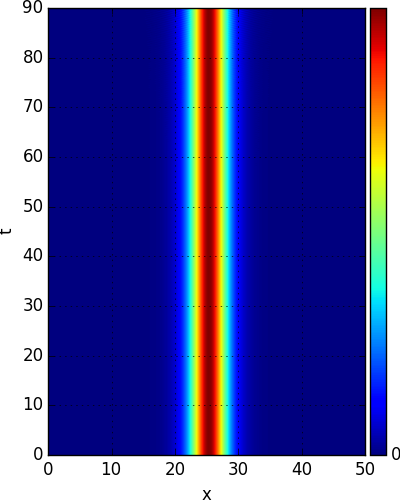
\includegraphics[width=.19\textwidth]{cqcglReq1T90}
    (2)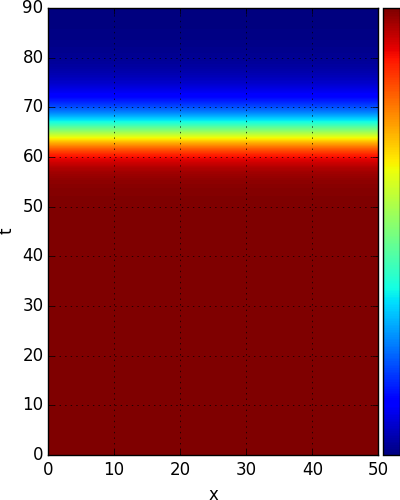
\includegraphics[width=.19\textwidth]{cqcglReq2T90}
    (3)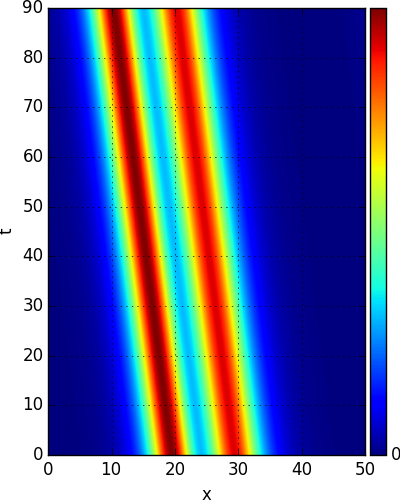
\includegraphics[width=.19\textwidth]{cqcglReq3T90}
    (4)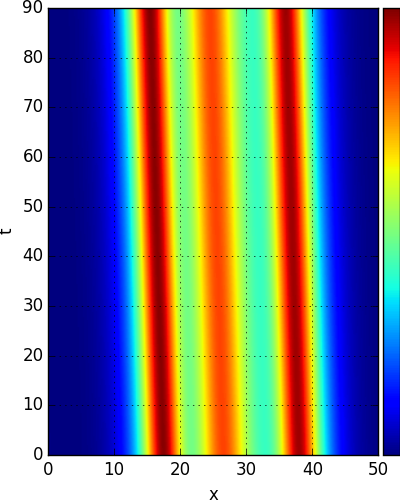
\includegraphics[width=.19\textwidth]{cqcglReq4T90}\\
    (5)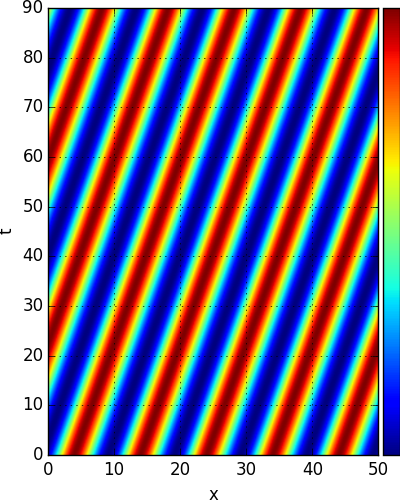
\includegraphics[width=.19\textwidth]{cqcglReq5T90}
    (6)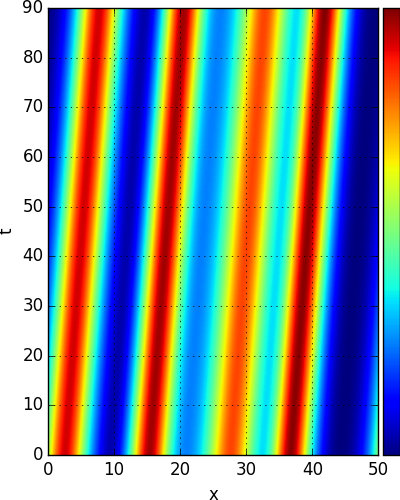
\includegraphics[width=.19\textwidth]{cqcglReq6T90}
    (7)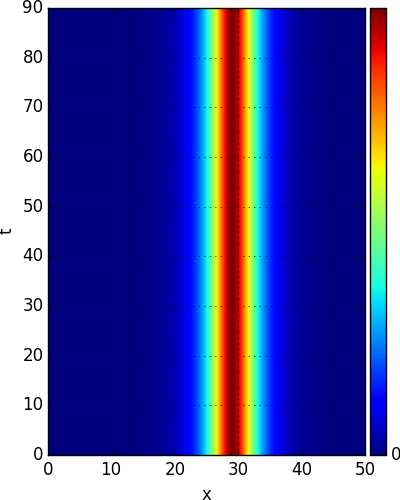
\includegraphics[width=.19\textwidth]{cqcglReq7T90}
    (8)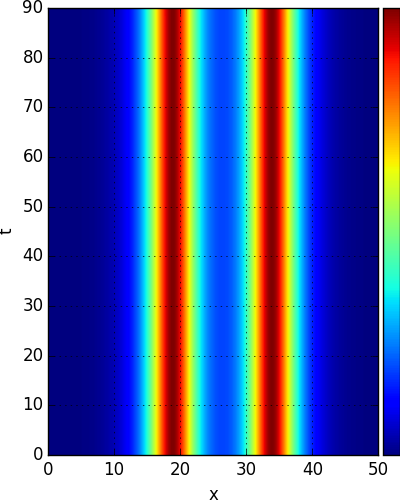
\includegraphics[width=.19\textwidth]{cqcglReq8T90}\\
    (9)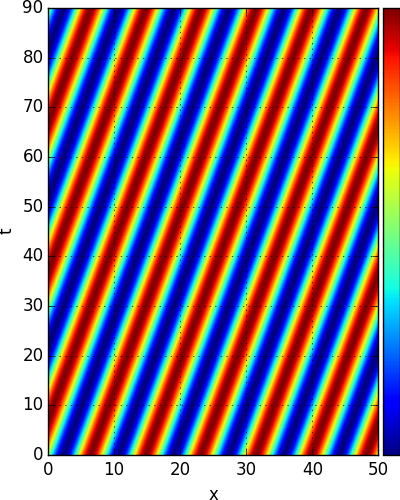
\includegraphics[width=.19\textwidth]{cqcglReq9T90}
   (10)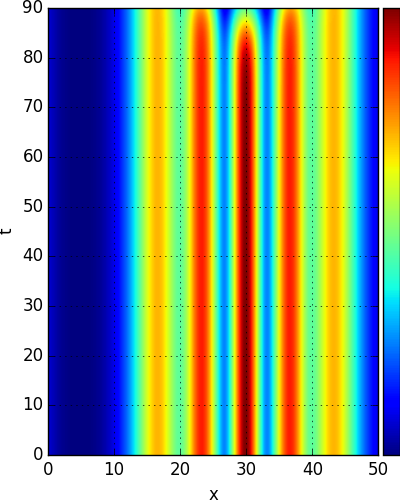
\includegraphics[width=.19\textwidth]{cqcglReq10T90}
   (11)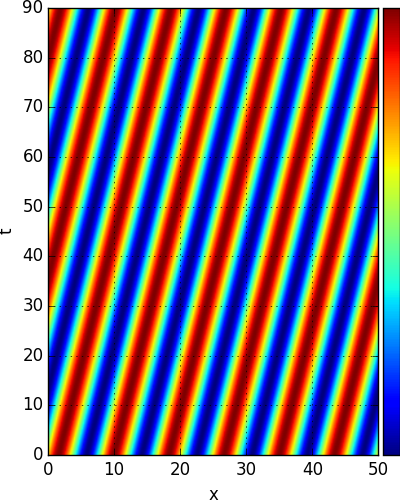
\includegraphics[width=.19\textwidth]{cqcglReq11T90}
   (12)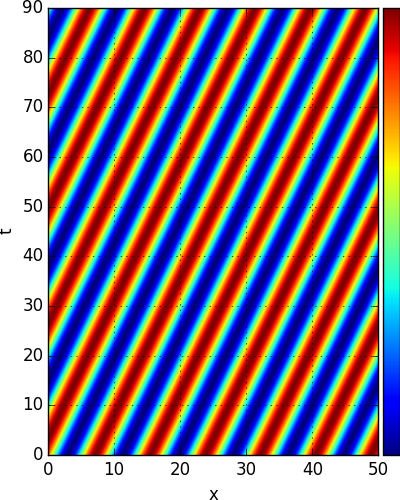
\includegraphics[width=.19\textwidth]{cqcglReq12T90}
    \label{fig:cqcglReqSet}
  \end{figure}

  \begin{figure}[h]
    \centering
    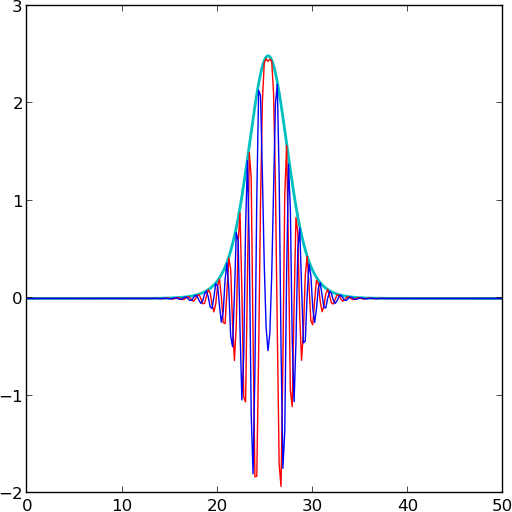
\includegraphics[width=0.35\textwidth]{req1Config} \hfill
    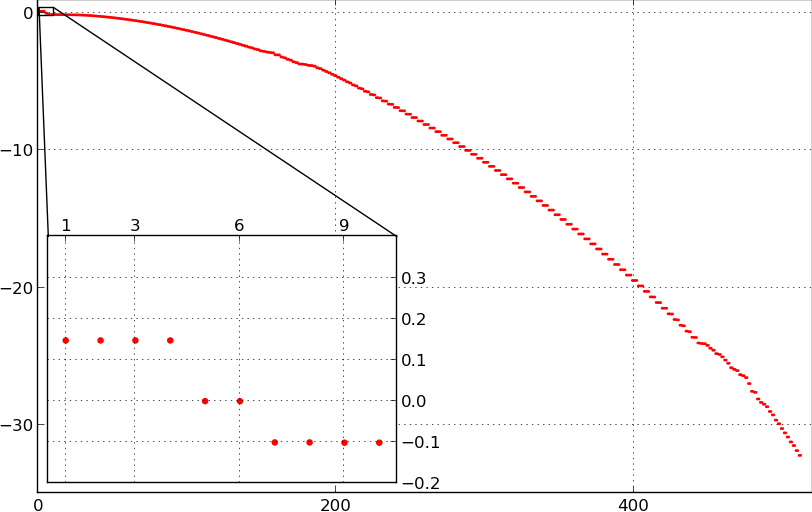
\includegraphics[width=0.55\textwidth]{req1Stability}
    \label{fig:req1Config}
  \end{figure}

  \begin{table}
    \centering
    \begin{tabular}{c | c}
      index & $\lambda$ \\
      \hline
      1,2    &    0.1474653 $\pm$      17.2375582i\\
      3,4    &    0.1474643 $\pm$      17.2375572i\\
      5    &    -7.21620620e-14             \\
      6    &     -1.86242571e-13  \\
      7,8    &   -0.1002241 $\pm$      17.6645298i\\
      9,10    &   -0.1008975 $\pm$      17.6556189i\\
      \hline
    \end{tabular}
    \label{tab:req1Stability}
  \end{table}

  \begin{figure}[h]
    \centering
    (a)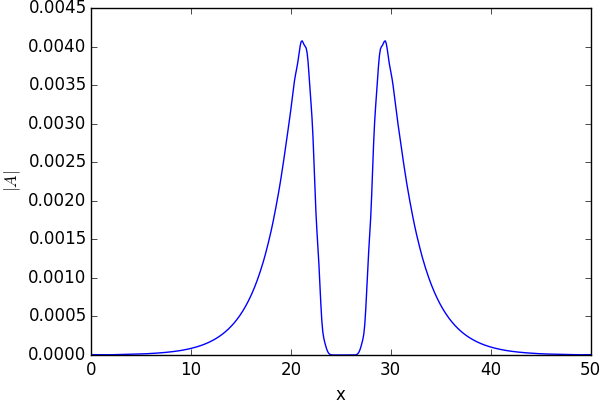
\includegraphics[width=0.4\textwidth]{cqcglReq1V1Real}
    (b)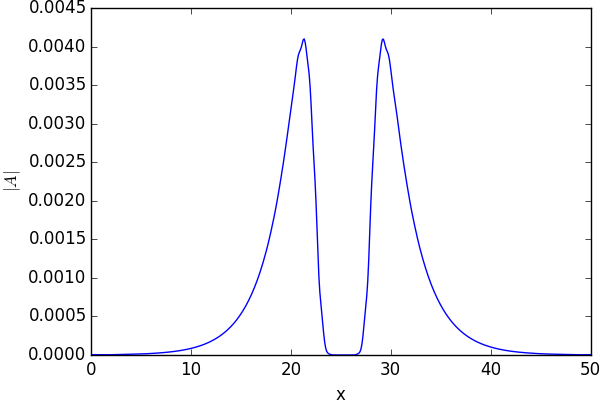
\includegraphics[width=0.4\textwidth]{cqcglReq1V1Imag} \\
    (c)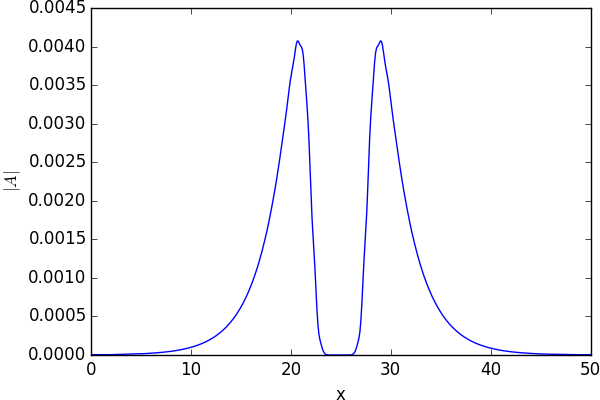
\includegraphics[width=0.4\textwidth]{cqcglReq1ReflectV1Real}
    (d)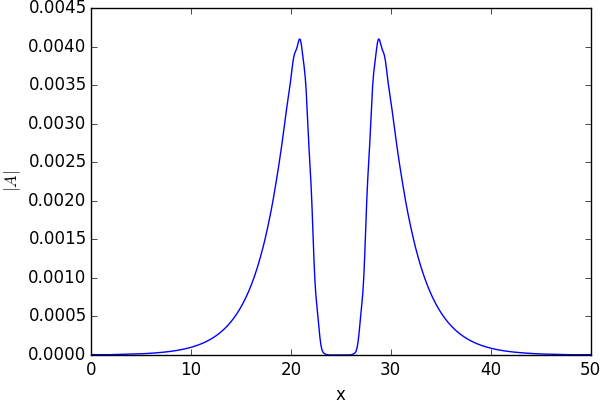
\includegraphics[width=0.4\textwidth]{cqcglReq1ReflectV1Imag}
    \label{fig:req1eigenvectors}
  \end{figure}

\end{frame}

\begin{frame}[allowframebreaks]
  \frametitle{\small{symmetry reduction in \cqcGLe}}

  \textbf{continuous symmetry} : $g(\theta,\phi) = g_\tau(\theta)g_\rho(\phi)$.

  \beq
  a_k(t) \to a_k(t)e^{i(k\theta + \phi)}
  \ee{eq:ft}


  \[
    Im(a_1) = Im(a_{-1}) = 0
  \]

  \beq
  \phi_s = \frac{1}{2}(\alpha_{1}+\alpha_{-1}) \,, \quad
  \theta_s = \frac{1}{2}(\alpha_{1} - \alpha_{-1}) \,.
  \ee{eq:cqcglPhaseAngle}

  \textbf{reflection symmetry} : $a_k \to a_{-k}$.

  \begin{equation}
    (b_0, c_0, b_1, c_1, b_2, c_2, \cdots, b_{-1}, c_{-1})
    \Rightarrow
    (b_0, c_0, b_{-1}, c_{-1}, b_{-2}, c_{-2}, \cdots, b_{1}, c_{1})
    \label{eq:reflectFullStateSpace}
  \end{equation}

  \begin{align}
    & (b_0, c_0, b_1, c_1, b_2, c_2, \cdots, b_{-1}, c_{-1})
      \Rightarrow \nonumber \\
    & (b_0, c_0, \frac{b_1-b_{-1}}{2}, \frac{c_1-c_{-1}}{2}, \frac{b_2-b_{-2}}{2},
      \frac{c_2-c_{-2}}{2}, \cdots,
      \frac{b_1+b_{-1}}{2}, \frac{c_1+c_{-1}}{2})
      \label{eq:reflectStep1}
  \end{align}

  \begin{align}
    & (b_0, c_0, p_1, q_1, p_2, q_2, \cdots, q_{N/2-1}, p_{-N/2+1}, \cdots, p_{-1}, q_{-1})
      \Rightarrow \nonumber \\
    & (b_0, c_0, r_1, s_1, r_2, s_2, \cdots, s_{N/2-1}, p_{-N/2+1}, \cdots, p_{-1}, q_{-1})
      \label{eq:reflectStep2}
  \end{align}

  \[
    r_1 = \frac{p_1^2-q_1^2}{\sqrt{p_1^2+q_1^2}}\,,
    s_1 = \frac{p_1 q_1}{\sqrt{p_1^2+q_1^2}} \,,
    r_2 = \frac{q_1 p_2}{\sqrt{q_1^2+p_2^2}} \,,
    s_2 = \frac{p_2 q_2}{\sqrt{p_2^2+q_2^2}} \,,
    \cdots
  \]

  \begin{equation}
    (b_0, c_0, r_2, \cdots, r_{N/2-1}, p_{-N/2+2}, q_{-N/2+2}, \cdots, p_{-2}, q_{-2})
    \Rightarrow
    (t_1, t_2, \cdots, t_{N-2})
    \label{eq:reduce2ndReflection}
  \end{equation}
  \[
    t_1 = \frac{b_0^2-c_0^2}{\sqrt{b_0^2+c_0^2}}\,,
    t_2 = \frac{b_0 c_0}{\sqrt{b_0^2+c_0^2}} \,,
    t_3 = \frac{r_2 c_0}{\sqrt{r_2^2+c_0^2}} \,,
    t_3 = \frac{r_3 r_2}{\sqrt{r_3^2+r_2^2}} \,,
    \cdots
  \]

  \begin{figure}[h]
  \centering
  \begin{subfigure}{.23\linewidth}
    \centering
    \captionsetup{justification=centering}
    \caption{}
    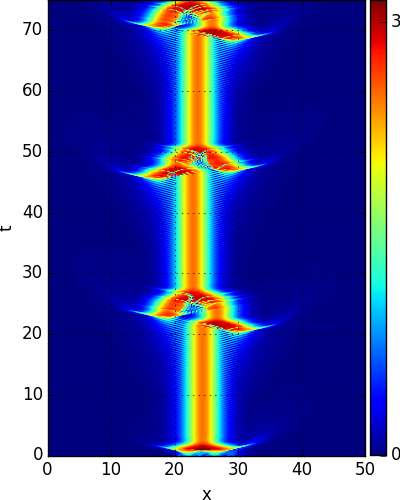
\includegraphics[width=\textwidth]{cqcglStateSpaceReflectT75h005}
    \label{}
  \end{subfigure}
  \begin{subfigure}{.23\linewidth}
    \centering
    \captionsetup{justification=centering}
    \caption{}
    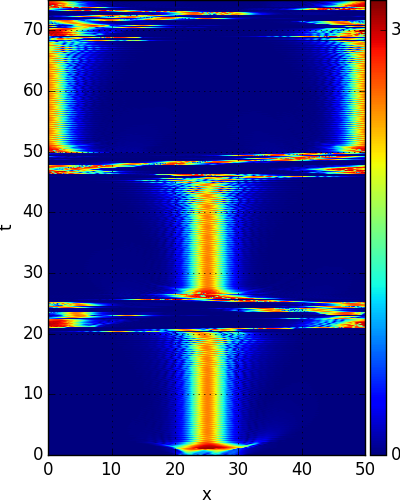
\includegraphics[width=\textwidth]{cqcglSliceUnwrappedReflectT75h005}
    \label{}
  \end{subfigure}
  \begin{subfigure}{.23\linewidth}
    \centering
    \captionsetup{justification=centering}
    \caption{}
    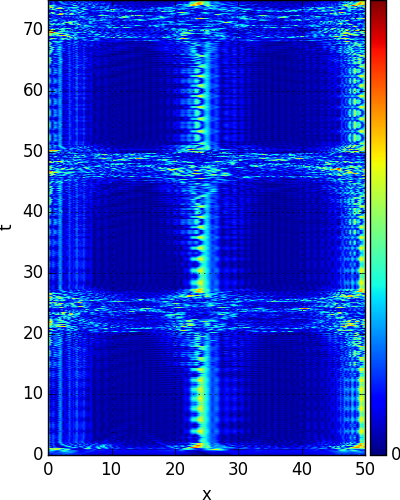
\includegraphics[width=\textwidth]{cqcglAllReduceT75h005}
    \label{}
  \end{subfigure}
  \label{fig:cqcglReduceSymT75h005}
\end{figure}

\end{frame}

\section{Future Plan}

\begin{frame}
  \frametitle{future research}

  \begin{itemize}
    \setlength\itemsep{4em}
  \item Dimension of Inertial Manifold Continued.
    \vspace{1em}

    \cGLe, 2-d or 3-d Navier-Stokes, etc.

  \item Cycle expansion in \cqcGLe.
    \vspace{1em}

    periodic orbits, symbolic dynamics, cycle expansion of spectral determinant, etc.

  \end{itemize}
\end{frame}


\begin{frame}[allowframebreaks]
  \frametitle{References}
  \scriptsize{\bibliographystyle{apalike}}
  \bibliography{../../../../bibtex/siminos}
\end{frame}

\usebackgroundtemplate
{
  
\includegraphics[width=\paperwidth,height=\paperheight]{lastpage.jpg}%
}
\begin{frame}

  \centering{ \huge Thank you for the time !}

  \vspace{2em}

  \centering{ \huge Any questions ?}

\end{frame}


\usebackgroundtemplate
{
  
\includegraphics[width=\paperwidth,height=\paperheight]{background.jpg}%
}



\end{document}
